\documentclass[11pt,letterpaper,landscape]{article}

\usepackage[margin=1.0cm]{geometry}
\usepackage{tikz}
\usetikzlibrary{arrows.meta,positioning,fit,calc}
\pagestyle{empty}

\tikzset{
  block/.style={draw, rounded corners=2pt, align=center, minimum width=3.0cm,
    minimum height=1.15cm, fill=gray!7, font=\sffamily\small},
  ic/.style={draw, rounded corners=2pt, align=center, minimum width=3.1cm,
    minimum height=1.35cm, fill=blue!7, font=\sffamily\small},
  part/.style={draw, rounded corners=2pt, align=left, minimum width=3.2cm,
    minimum height=1.1cm, fill=white, font=\sffamily\scriptsize},
  note/.style={align=left, font=\sffamily\scriptsize},
  sig/.style={-Latex, thick},
  bus/.style={thick},
  group/.style={draw, rounded corners=4pt, dashed, inner sep=7pt}
}

\newcommand{\titlebar}[1]{%
  \begin{center}
    {\Large\sffamily\bfseries #1}\\[-1mm]
    {\sffamily\small IE0413 - Generacion de formas de onda. Valores para $X=2$, $Y=2$, $Z=9$.}
  \end{center}
  \vspace{2mm}
}

\begin{document}

\titlebar{Esquematico general recomendado}

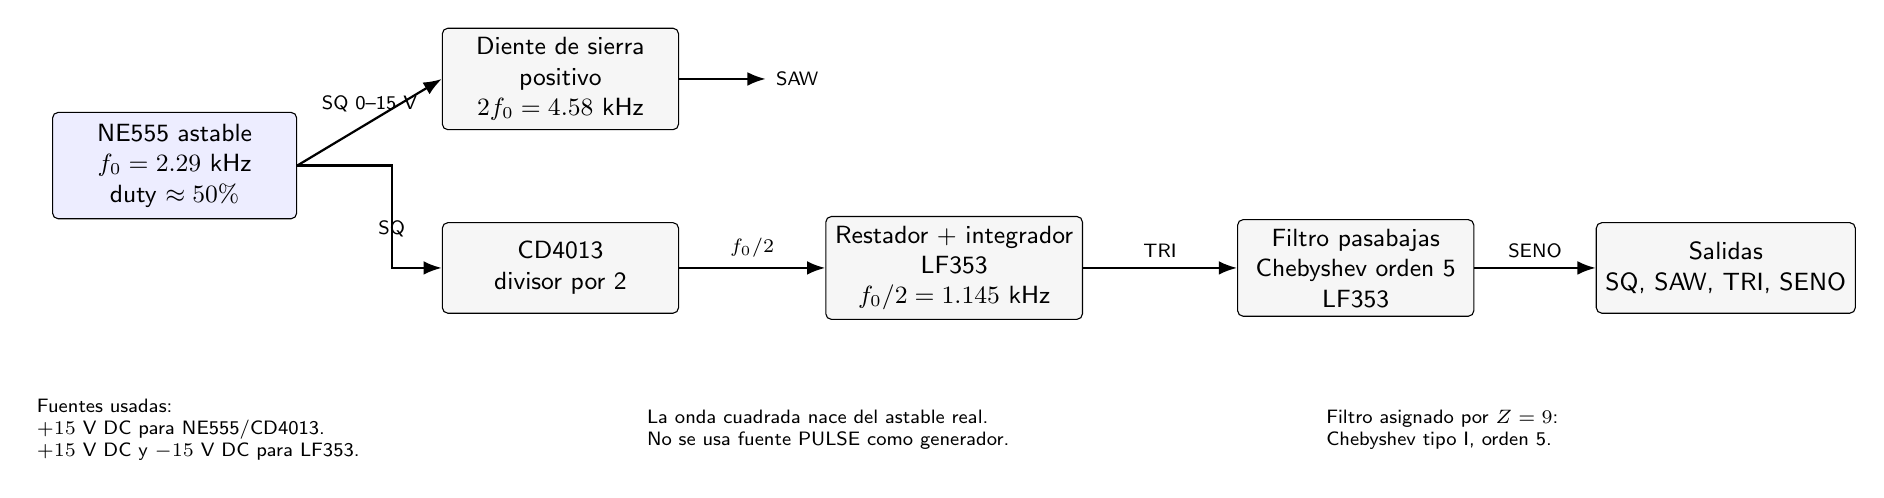
\begin{tikzpicture}[x=1cm,y=1cm]
  \node[ic] (osc) at (1.5,4.7) {NE555 astable\\$f_0=2.29$ kHz\\duty $\approx 50\%$};
  \node[block] (saw) at (6.4,5.8) {Diente de sierra\\positivo\\$2f_0=4.58$ kHz};
  \node[block] (div) at (6.4,3.4) {CD4013\\divisor por 2};
  \node[block] (tri) at (11.4,3.4) {Restador + integrador\\LF353\\$f_0/2=1.145$ kHz};
  \node[block] (filt) at (16.5,3.4) {Filtro pasabajas\\Chebyshev orden 5\\LF353};
  \node[block] (outs) at (21.2,3.4) {Salidas\\SQ, SAW, TRI, SENO};

  \draw[sig] (osc.east) -- node[above, font=\sffamily\scriptsize]{SQ 0--15 V} (saw.west);
  \draw[sig] (osc.east) -- ++(1.2,0) |- node[pos=0.22, below, font=\sffamily\scriptsize]{SQ} (div.west);
  \draw[sig] (div.east) -- node[above, font=\sffamily\scriptsize]{$f_0/2$} (tri.west);
  \draw[sig] (tri.east) -- node[above, font=\sffamily\scriptsize]{TRI} (filt.west);
  \draw[sig] (filt.east) -- node[above, font=\sffamily\scriptsize]{SENO} (outs.west);
  \draw[sig] (saw.east) -- ++(1.1,0) node[right, font=\sffamily\scriptsize]{SAW};

  \node[note] at (1.8,1.35) {Fuentes usadas:\\$+15$ V DC para NE555/CD4013.\\$+15$ V DC y $-15$ V DC para LF353.};
  \node[note] at (9.8,1.35) {La onda cuadrada nace del astable real.\\No se usa fuente PULSE como generador.};
  \node[note] at (17.6,1.35) {Filtro asignado por $Z=9$:\\Chebyshev tipo I, orden 5.};
\end{tikzpicture}

\newpage
\titlebar{Detalle A: oscilador astable y diente de sierra}

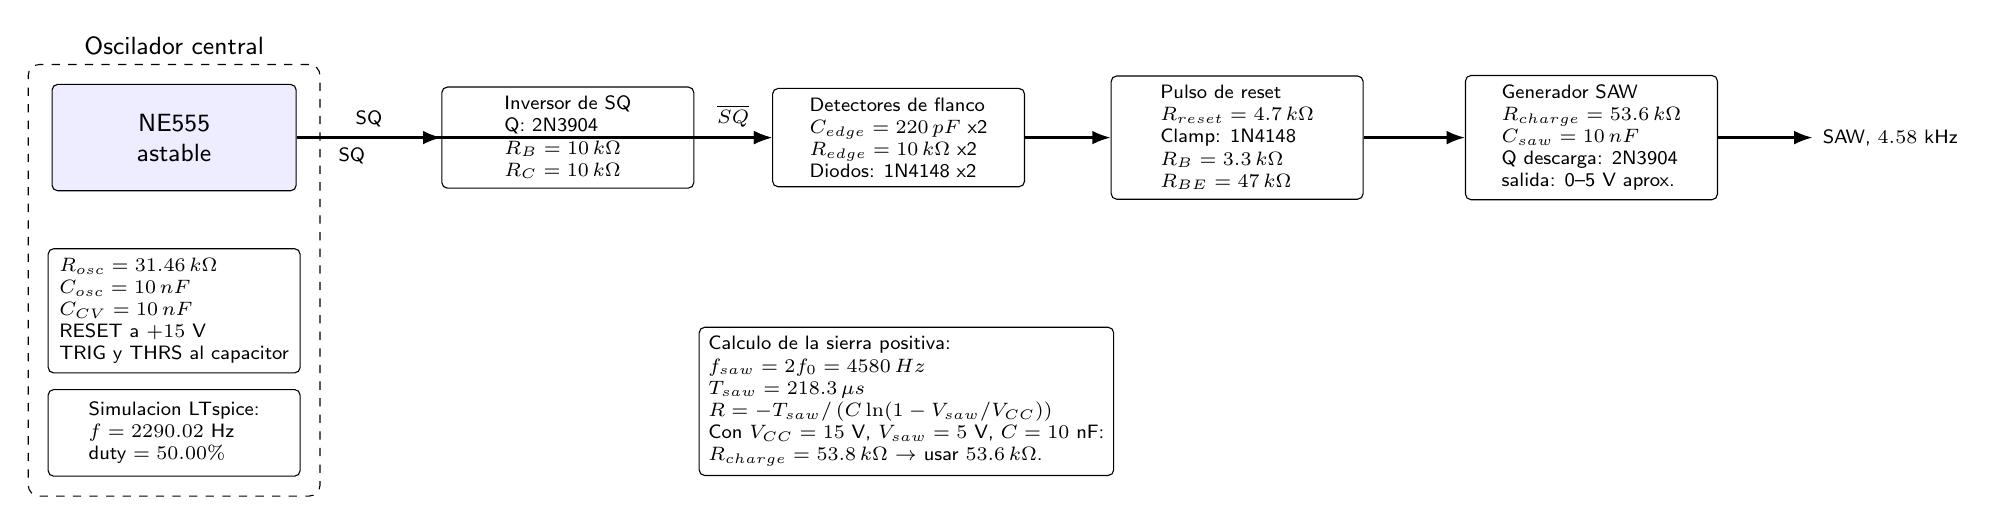
\begin{tikzpicture}[x=1cm,y=1cm]
  \node[ic] (u555) at (2.0,5.1) {NE555\\astable};
  \node[part] (oscvals) at (2.0,2.9) {
    $R_{osc}=31.46\,k\Omega$\\
    $C_{osc}=10\,nF$\\
    $C_{CV}=10\,nF$\\
    RESET a $+15$ V\\
    TRIG y THRS al capacitor
  };
  \node[part] (oscmeas) at (2.0,1.35) {
    Simulacion LTspice:\\
    $f=2290.02$ Hz\\
    duty $=50.00\%$
  };
  \node[group, fit=(u555)(oscvals)(oscmeas), label={[font=\sffamily\small]above:Oscilador central}] {};

  \node[part] (inv) at (7.0,5.1) {
    Inversor de SQ\\
    Q: 2N3904\\
    $R_B=10\,k\Omega$\\
    $R_C=10\,k\Omega$
  };
  \node[part] (edges) at (11.2,5.1) {
    Detectores de flanco\\
    $C_{edge}=220\,pF$ x2\\
    $R_{edge}=10\,k\Omega$ x2\\
    Diodos: 1N4148 x2
  };
  \node[part] (reset) at (15.5,5.1) {
    Pulso de reset\\
    $R_{reset}=4.7\,k\Omega$\\
    Clamp: 1N4148\\
    $R_B=3.3\,k\Omega$\\
    $R_{BE}=47\,k\Omega$
  };
  \node[part] (sawcap) at (20.0,5.1) {
    Generador SAW\\
    $R_{charge}=53.6\,k\Omega$\\
    $C_{saw}=10\,nF$\\
    Q descarga: 2N3904\\
    salida: 0--5 V aprox.
  };

  \draw[sig] (u555.east) -- node[above, font=\sffamily\scriptsize]{SQ} (inv.west);
  \draw[sig] (u555.east) -- ++(0.7,0) |- node[pos=0.25, below, font=\sffamily\scriptsize]{SQ} (edges.west);
  \draw[sig] (inv.east) -- node[above, font=\sffamily\scriptsize]{$\overline{SQ}$} (edges.west);
  \draw[sig] (edges.east) -- (reset.west);
  \draw[sig] (reset.east) -- (sawcap.west);
  \draw[sig] (sawcap.east) -- ++(1.2,0) node[right, font=\sffamily\scriptsize]{SAW, $4.58$ kHz};

  \node[part] (formula) at (11.3,1.75) {
    Calculo de la sierra positiva:\\
    $f_{saw}=2f_0=4580\,Hz$\\
    $T_{saw}=218.3\,\mu s$\\
    $R=-T_{saw}/\left(C\ln(1-V_{saw}/V_{CC})\right)$\\
    Con $V_{CC}=15$ V, $V_{saw}=5$ V, $C=10$ nF:\\
    $R_{charge}=53.8\,k\Omega$ $\rightarrow$ usar $53.6\,k\Omega$.
  };
\end{tikzpicture}

\newpage
\titlebar{Detalle B: triangular y filtro activo}

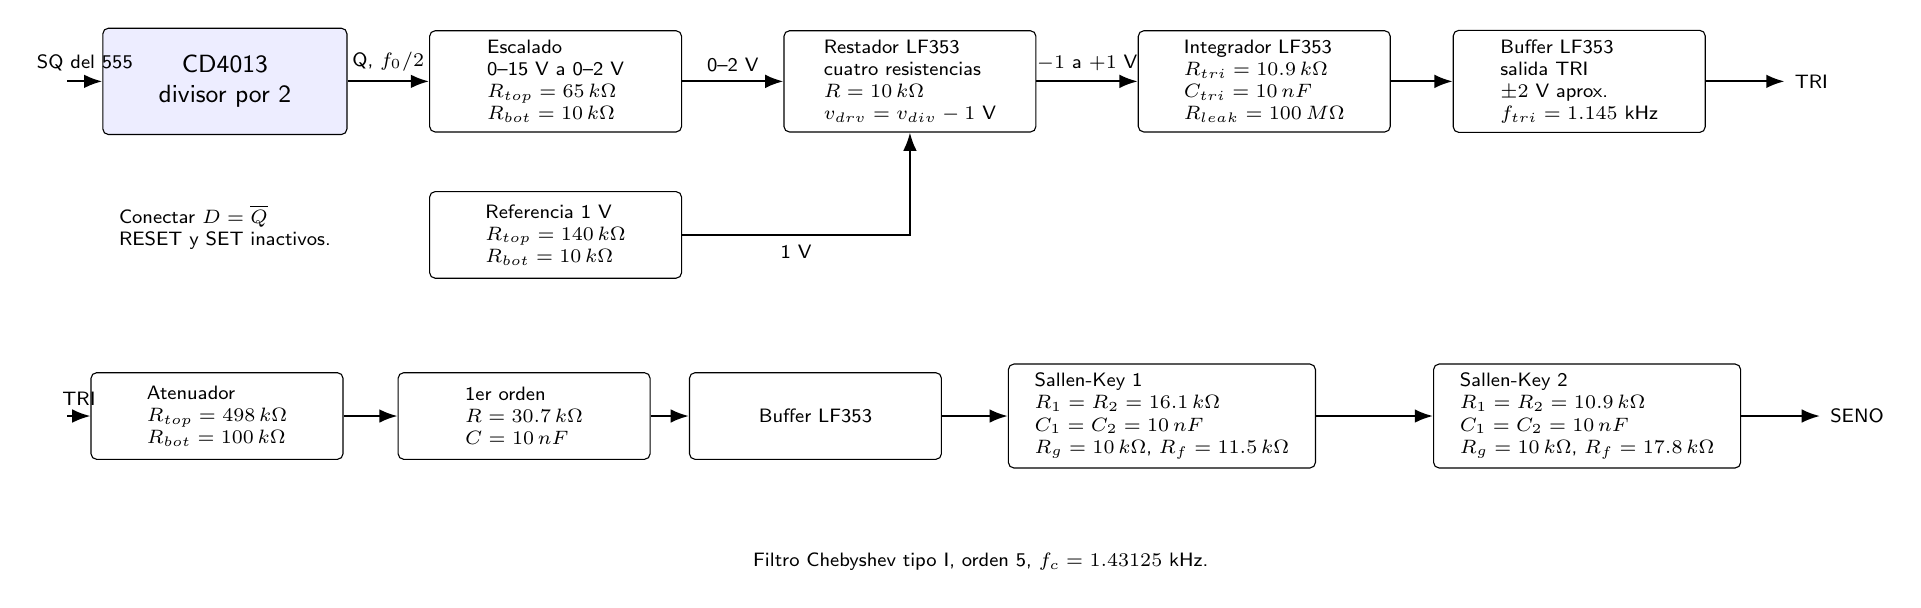
\begin{tikzpicture}[x=1cm,y=1cm]
  % Triangular chain
  \node[ic] (cd) at (1.8,5.5) {CD4013\\divisor por 2};
  \node[part] (divscale) at (6.0,5.5) {
    Escalado\\
    0--15 V a 0--2 V\\
    $R_{top}=65\,k\Omega$\\
    $R_{bot}=10\,k\Omega$
  };
  \node[part] (ref) at (6.0,3.55) {
    Referencia 1 V\\
    $R_{top}=140\,k\Omega$\\
    $R_{bot}=10\,k\Omega$
  };
  \node[part] (sub) at (10.5,5.5) {
    Restador LF353\\
    cuatro resistencias\\
    $R=10\,k\Omega$\\
    $v_{drv}=v_{div}-1$ V
  };
  \node[part] (integ) at (15.0,5.5) {
    Integrador LF353\\
    $R_{tri}=10.9\,k\Omega$\\
    $C_{tri}=10\,nF$\\
    $R_{leak}=100\,M\Omega$
  };
  \node[part] (tribuf) at (19.0,5.5) {
    Buffer LF353\\
    salida TRI\\
    $\pm2$ V aprox.\\
    $f_{tri}=1.145$ kHz
  };

  \draw[sig] (-0.2,5.5) -- node[above, font=\sffamily\scriptsize]{SQ del 555} (cd.west);
  \draw[sig] (cd.east) -- node[above, font=\sffamily\scriptsize]{Q, $f_0/2$} (divscale.west);
  \draw[sig] (divscale.east) -- node[above, font=\sffamily\scriptsize]{0--2 V} (sub.west);
  \draw[sig] (ref.east) -| node[pos=0.25, below, font=\sffamily\scriptsize]{1 V} (sub.south);
  \draw[sig] (sub.east) -- node[above, font=\sffamily\scriptsize]{$-1$ a $+1$ V} (integ.west);
  \draw[sig] (integ.east) -- (tribuf.west);
  \draw[sig] (tribuf.east) -- ++(1.0,0) node[right, font=\sffamily\scriptsize]{TRI};
  \node[note] at (1.8,3.65) {Conectar $D=\overline{Q}$\\RESET y SET inactivos.};

  % Filter chain
  \node[part] (att) at (1.7,1.25) {
    Atenuador\\
    $R_{top}=498\,k\Omega$\\
    $R_{bot}=100\,k\Omega$
  };
  \node[part] (fo) at (5.6,1.25) {
    1er orden\\
    $R=30.7\,k\Omega$\\
    $C=10\,nF$
  };
  \node[part] (buf) at (9.3,1.25) {Buffer LF353};
  \node[part, minimum width=3.9cm] (sk1) at (13.7,1.25) {
    Sallen-Key 1\\
    $R_1=R_2=16.1\,k\Omega$\\
    $C_1=C_2=10\,nF$\\
    $R_g=10\,k\Omega$, $R_f=11.5\,k\Omega$
  };
  \node[part, minimum width=3.9cm] (sk2) at (19.1,1.25) {
    Sallen-Key 2\\
    $R_1=R_2=10.9\,k\Omega$\\
    $C_1=C_2=10\,nF$\\
    $R_g=10\,k\Omega$, $R_f=17.8\,k\Omega$
  };

  \draw[sig] (-0.2,1.25) -- node[above, font=\sffamily\scriptsize]{TRI} (att.west);
  \draw[sig] (att.east) -- (fo.west);
  \draw[sig] (fo.east) -- (buf.west);
  \draw[sig] (buf.east) -- (sk1.west);
  \draw[sig] (sk1.east) -- (sk2.west);
  \draw[sig] (sk2.east) -- ++(1.0,0) node[right, font=\sffamily\scriptsize]{SENO};

  \node[note] at (11.4,-0.6) {Filtro Chebyshev tipo I, orden 5, $f_c=1.43125$ kHz.};
\end{tikzpicture}

\end{document}
